\chapter{Data understanding}
This chapter gives an overview of basic terminology and explains some common techniques of data understanding. Data understanding provides general information about the data: allows us to have a view of the different attributes and how they relate to each other, highlights the presence of wrong or missing values, and so on.

\section{What is data?}

A \textbf{dataset} is a collection of data objects (a.k.a. records, samples, points, patterns, etc.).
A \textbf{data object} is a collection of $n$ attributes (a.k.a. variables, fields, features, etc.). The number of attributes in a data object is called its \textbf{dimensionality}.
An \textbf{attribute} is a property or characteristic of an object that can vary, either from one object to another, or from one time to another. 

\section{Types of attribute}

\BoxDef{Categorical (Qualitative)}{
Attributes that can take one of a limited number of values.
\begin{itemize}
    \item \textbf{Nominal}: attribute values belong to a finite domain of names. E.g.: IDs, zip-codes, eye color, gender;

    \item \textbf{Ordinal}: attribute values belong to a finite domain where a meaningful order can be seen. E.g.: scale of hardness of minerals, grades, street number.
\end{itemize}
}

\BoxDef{Numeric (Quantitative)}{
Attributes that represents a measurable quantity.
\begin{itemize}
    \item \textbf{Interval}: values correspond to measures done on a scale of equal sized units; i.e, a unit of measurement exists. E.g.: calendar data, temperature (in °C or °F);

    \item \textbf{Ratio scaled}: values are expressed by specifying by what order of magnitude they are larger/smaller than some unit of measurement. E.g: distances, temperature (in K).
\end{itemize}
}

\BoxDef{Binary attributes}{
Nominal attributes with only 2 possible outcomes.

\begin{itemize}
    \item \textbf{Symmetric binary}: both outcomes are equally important;
    \item \textbf{Asymmetric binary}: one outcome is more important than the other; the former is typically associated with the value 1.
\end{itemize}
}

\BoxDef{Attributes by number of values}{
Attributes can also be classified as:
\begin{itemize}
    \item \textbf{Discrete}: attribute has a finite (or countably infinite) set of values. They are often represented by integer variables;
    
    \item \textbf{Continuous}: attribute has real numbers as values. They are often represented by floating-point variables.
\end{itemize}
}
The type of attribute can be determined by which of the following operations/properties apply:

\begin{table}[h]
    \centering
    \begin{tabular}{l|l}
        (1) Distinctness & $=, \neq$\\
        (2) Order & $<, >$\\
        (3) Differences are meaningful & $+, -$\\
        (4) Ratios are meaningful & $*, /$\\
    \end{tabular}
\end{table}

\textbf{Nominal}: (1)

\textbf{Ordinal}: (1), (2)

\textbf{Interval}: (1), (2), (3)

\textbf{Ratio}: (1), (2), (3), (4)


\section{Types of dataset}

There are many types of datasets. The following list contains the most commonly used, but it's not exhaustive.

\begin{itemize}
    \item \textbf{Record data}: collection of records (i.e., data objects), each of which is a collection of data fields (i.e., attributes). Record data is usually stored in flat files or relational databases.

    Types include: simple record data, data matrix, transaction data, document-
    term matrix

    \item \textbf{Graph-based data}: used to represent actual graphs, or any data where the relationship between objects is relevant.

    \item \textbf{Ordered data}: the objects/attributes have spatio-temporal relationships.

    Types include: sequential transaction data, sequence data, time series data, spatial and spatio-temporal data.
\end{itemize}


\section{Data Quality}

In data mining, preventing data quality issues is near impossible. Instead, the focus is on detecting and correcting data quality issues, and using algorithms that can handle poor data quality. The first step is called data cleaning.

\subsection{Possible issues}

\paragraph{Measurement and data collection errors}
Omitted data-objects or values, or data-objects inappropriately included.

\paragraph{Noise and artifacts}
Noise is the addition of random error to a measurement. Artifacts are errors caused by a deterministic phenomenons.

\paragraph{Outliers}
Data values/objects that are very inconsistent with the rest. They're either caused by mistakes in measurements, or are actual legitimate measurements we may be interested in discovering. Whether they're the former or the latter, it's often useful to detect and eliminate all outliers from the dataset before analyzing the data, since they may skew certain calculations. The process of finding outliers is called \textbf{outlier detection}.

Single outlier attributes can be discovered by using box plots (for numerical attributes), or bar charts (for categorical attributes). Multidimensional attributes are typically discovered (visually) by using scatter plots and parallel coordinates plot, or by using cluster analysis techniques.

\paragraph{Missing values}
Missing values in one or more attributes of an object. The values may not have been collected to begin with, either because the user chose or forgot to input the data or because a sensor receiving the data broke, or they are intentionally left blank in some objects because they don't apply to those specific objects. Missing values are also not always explicitly indicated as such, and may instead be displayed as a default value or a 0.

\paragraph{Inconsistent data}
Inconsistency regarding either syntax (a value does not appear in the domain of that attribute), or semantic (the value is acceptable, but does not make sense when paired with the other attribute values of the same object).

\paragraph{Duplicate data}
Two or more objects are duplicates of each other. Can be caused by an input mistake, or can be legitimate values that just happen to be identical between objects.

\paragraph{Timeliness}
Data is not up to date.

\paragraph{Unbalanced data}
The dataset is heavily biased towards a certain type of object.

\section{Measures}

\subsection{Measuring the central tendency}

\BoxDef{Mean}{
The mean of a set of values is calculated as:
\begin{equation*}
    \textit{mean}(x) = \dfrac{1}{m} \sum_{i=1}^{m} x_i
\end{equation*}
}

\BoxDef{Median}{
The median of a set of values is the middle value if the number of elements is odd, else it's the average of the two middle values.
}

\BoxDef{Mode}{
The mode of a set of values is the value with the highest frequency. There may be multiple values with the same (highest) frequency; those are called bimodal, trimodal, ..., multimodal distributions. In case all values have the same frequency, then there is no mode.
}

\subsection{Measuring the dispersion}
The degree in which the data tends to spread is called the \textbf{dispersion}, or \textbf{variance}.

\BoxDef{Variance}{
Variance is calculated as:
\begin{equation*}
    \textit{var}(x) = \sigma_x^2(x) = \dfrac{\sum_{i=1}^m (x - \textit{mean}(x))^2}{m-1}
\end{equation*}
}

\BoxDef{Covariance}{
Covariance measures the join variability of two variables, showing how much the two variables are connected by a linear relationship. It's calculated as: 

\begin{equation*}
    \textit{cov}(x,y) = \dfrac{\sum_{i=1}^n (x_i - \textit{mean}(x))(y_i - \textit{mean}(y))}{n-1}
\end{equation*}

}

\BoxDef{Standard deviation}{
The standard deviation, $\sigma_x$, is calculated as:

\begin{equation*}
    \sigma_x = \sqrt{\sigma_x^2}
\end{equation*}

It measures how much the data spreads w.r.t the mean, so it should be used only when the mean is chosen as the measure of the center. When $\sigma = 0$, all the values are equal (i.e. there is no spread from the mean). When $\sigma > 0$, then there is spread.
}

\BoxDef{Range}{
It's the distance between the largest and the smallest values.
}

\section{Data visualization}

Visualizing data can be an useful and intuitive way to analyze it and detect general trends and patterns (including outliers).

\paragraph{Bar charts and histograms}

A \textbf{bar chart} is used to depict the frequency of \textbf{categorical} attributes. An \textbf{histogram} is used to depict the frequency of \textbf{numerical} attributes. The range of attributes is normally discretized into a fixed number of intervals, called \textbf{bins}.

\begin{figure}[h]
    \centering
    \begin{minipage}[b]{0.40\textwidth}
        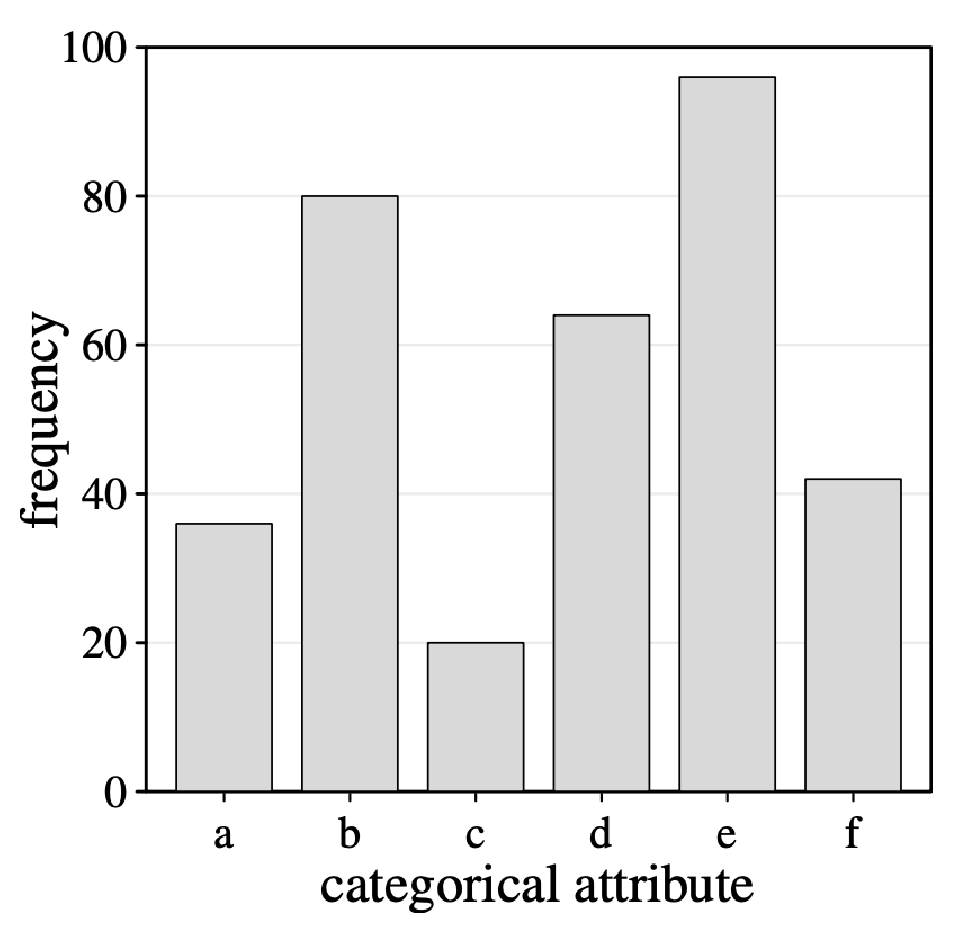
\includegraphics[width=\textwidth]{img/bar chart.png}
        \caption{A bar chart.}
    \end{minipage}
    \hfill
    \begin{minipage}[b]{0.45\textwidth}
        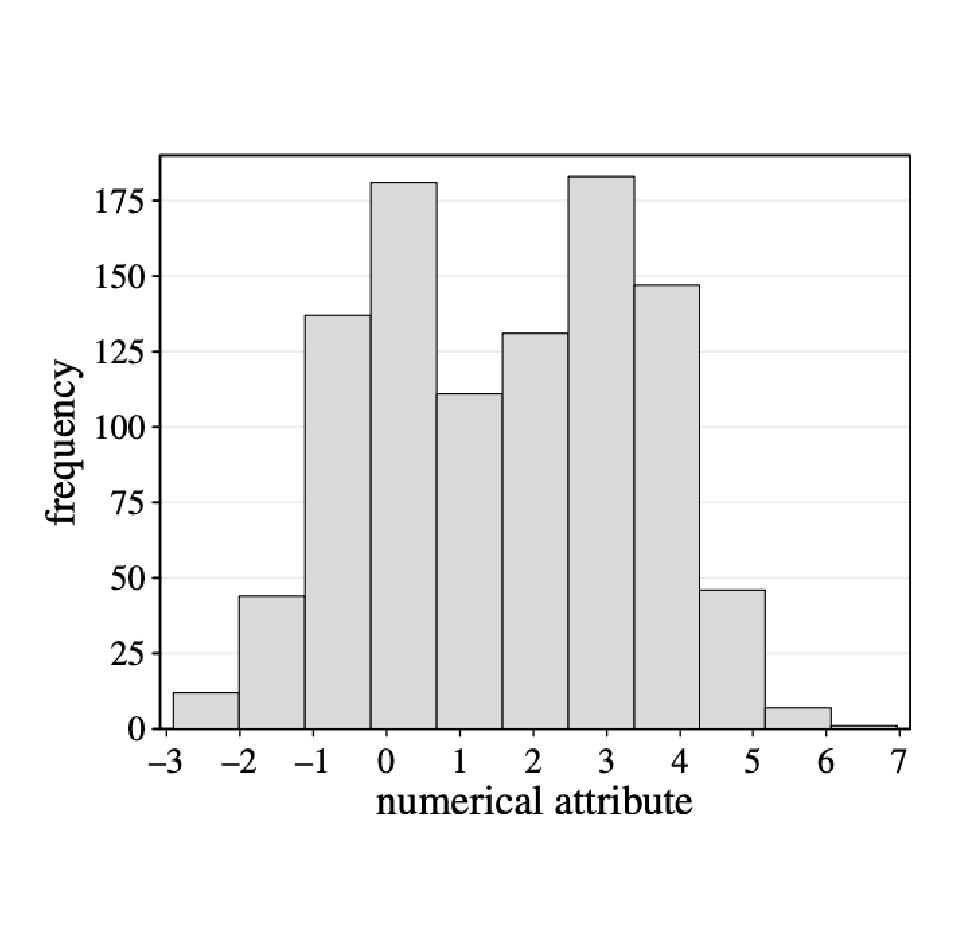
\includegraphics[width=\textwidth]{img/histogram.png}
        \caption{An histogram.}
    \end{minipage}
\end{figure}

\BoxDef{Sturges' rule}{
The number of bins, $k$, can be calculated using Sturges' rule:
\begin{equation*}
    k=\lceil{\log_2(n) + 1}\rceil
\end{equation*}
where $n$ is the number of data objects. This formula is especially suitable for data from normal distributions and from datasets of moderate size.
}

\BoxDef{Natural binning}{
A simple way of distributing values across bins is by using natural binning. Given $\delta$:
\begin{equation*}
    \delta = \dfrac{x_{max} - x_{min}}{k}    
\end{equation*}
then, element $x_j$ belongs to class $i$ if:
\begin{equation*}
    x_j \in [x_{min} + i*\delta, x_{min} + (i+1)*\delta]
\end{equation*}
}

\BoxDef{Equal frequency binning}{
Natural binning can generate an unbalanced distribution, where some bins may contain a lot more elements than others. The alternative is to calculate the frequency, $f$:
\begin{equation*}
    f = \dfrac{N}{k}
\end{equation*}
which determines how many elements must be contained in a single bin. Then, element $x_j$ belongs to class $i$ if:
\begin{equation*}
    i*f \leq j < (i+1)*f
\end{equation*}
}
This last method is not too useful to uncover interesting distribution of data, however.

\paragraph{Scatter plot}
A scatter plot is used to analyze the presence of clusters of points, outliers, and correlation between data points. Each pair of values plotted is treated as a pair of point coordinates that determine where the point will be displayed relative to the $x$ and $y$ axes. Scatter plots may be used to visualize data up to 3 dimensions, where each point has three coordinates, as to visualize three features at once.

Multiple scatter plots can be aggregated in a \textbf{scatter matrix} that combines multiple attributes at once.

\begin{figure}[h]
    \centering
    \begin{minipage}[b]{0.45\textwidth}
        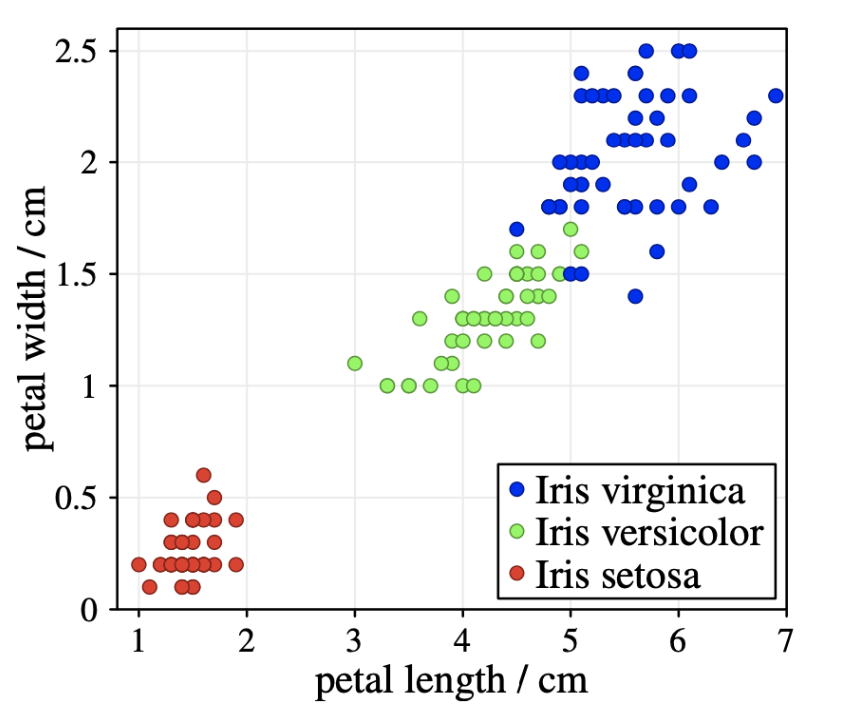
\includegraphics[width=\textwidth]{img/scatter plot.png}
        \caption{A scatter plot.}
    \end{minipage}
    \hfill
    \begin{minipage}[b]{0.47\textwidth}
        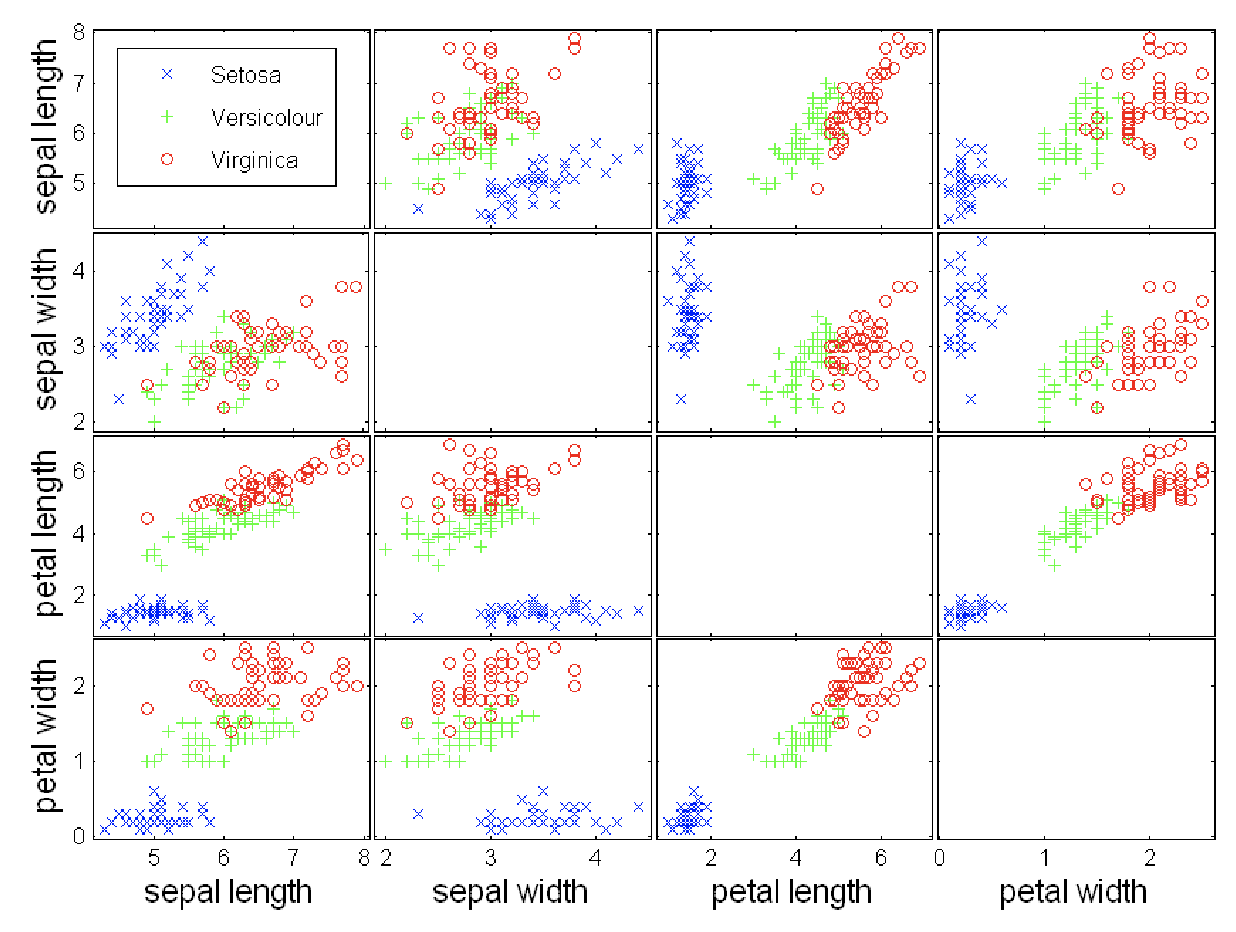
\includegraphics[width=\textwidth]{img/scatter matrix.png}
        \caption{A scatter matrix visualizing multiple scatter plots at once.}
    \end{minipage}
\end{figure}

\paragraph{Five-number summary and box plot}
A five number summary is done by determining five values, typically corresponding to:

\begin{itemize}
    \item $10^{th}$ percentile;
    \item $25^{th}$ percentile (or $1^{st}$ quartile);
    \item $50^{th}$ percentile (or $2^{nd}$ quartile, corresponding to the mean);
    \item $75^{th}$ percentile (or $3^{rd}$ quartile);
    \item $90^{th}$ percentile.
\end{itemize}

Once these values are calculated, the data can be visualized with a \textbf{box plot}. The $25^th$ and $75^{th}$ percentiles are the ends of the box, and the distance between the two is called the \textbf{interquartile range (IQR)}. The $10^{th}$ and $90^{th}$ percentile are instead called \textbf{whiskers}. This way of visualizing data is especially useful for discovering outliers.

\begin{figure}[h]
    \centering
    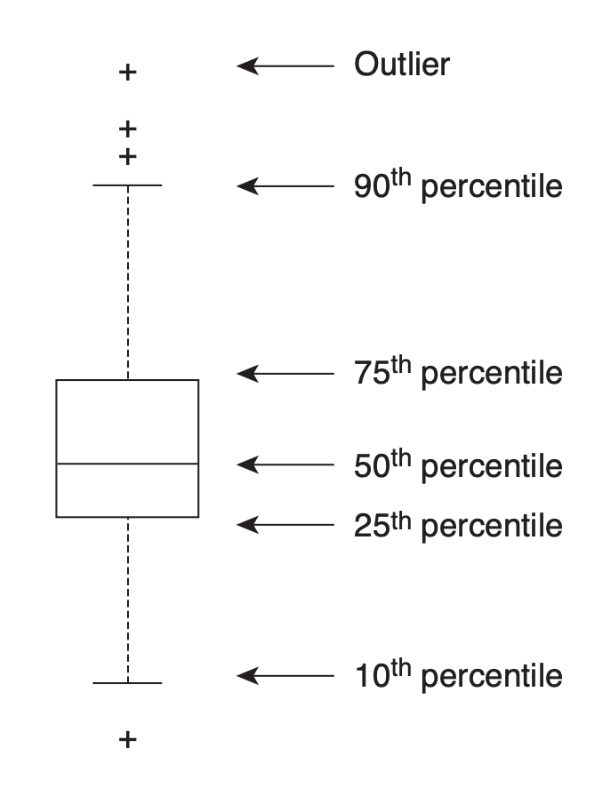
\includegraphics[width=0.4\linewidth]{img/box plot.png}
    \caption{A box plot.}
\end{figure}

\paragraph{Parallel coordinates plot}
This type of plot is often used to visualize attributes of high-dimensional data ($> 3$). Instead of using two perpendicular axes, this plot uses $n$ parallel axes (where $n$ is the number of attributes we want to visualize). The attribute values of each individual object are then plotted as points on each axis, forming a straight line. The resulting plot will contain a separate line for each object in the dataset. Areas with a denser number of lines suggest some correlation between the objects corresponding to those lines.

\begin{figure}[h]
    \centering
    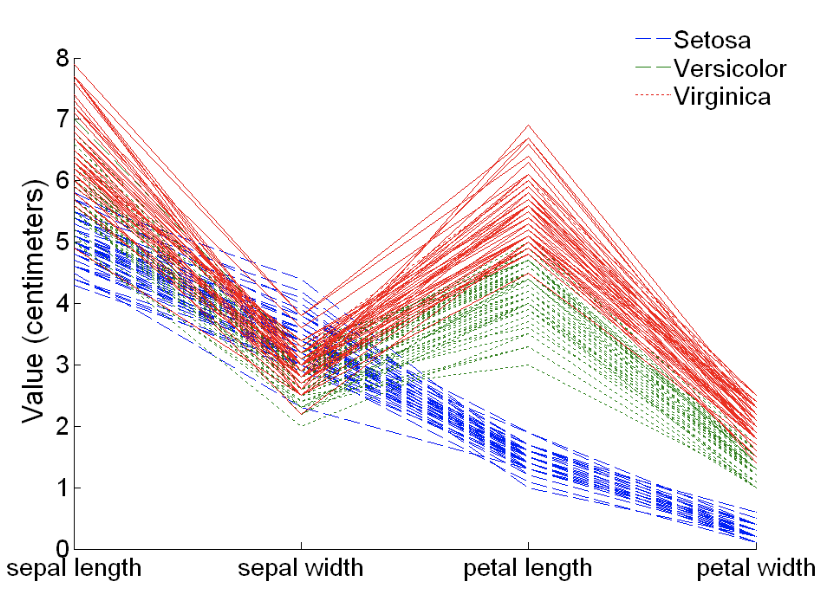
\includegraphics[width=0.4\linewidth]{img/Parallel coord plot.png}  
    \caption{A parallel coordinates plot.}
\end{figure}

\paragraph{Data matrix plot}
Matrix plots are useful to visualize data sorted according to class. The attribute values are normalized to prevent one attribute from dominating the plot. A common type of data matrix plot is the distance matrix, which visualizes the value of the standard deviation $\sigma$ for each value.

\begin{figure}[h]
    \centering
    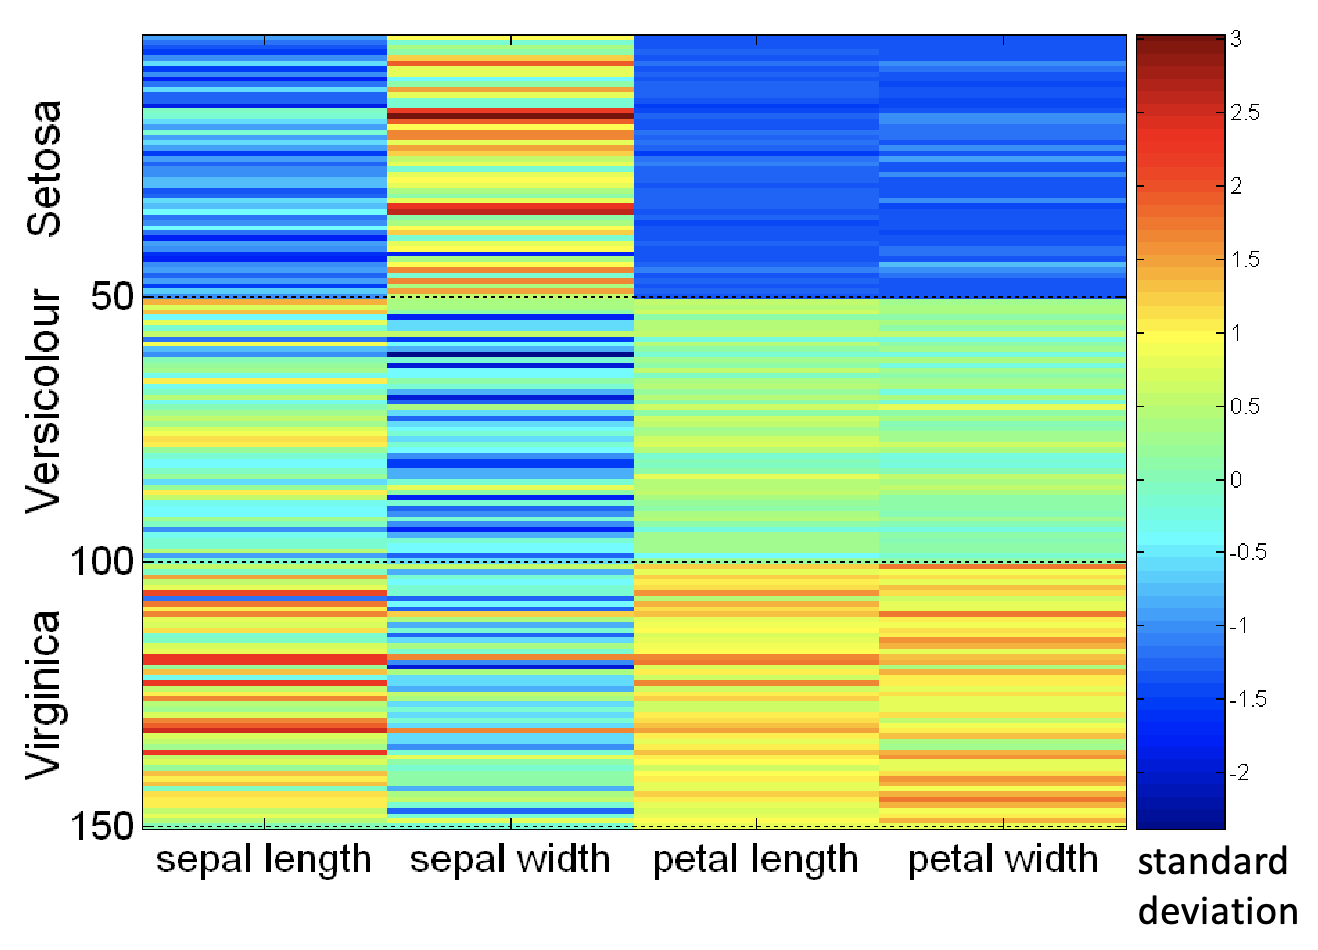
\includegraphics[width=0.4\linewidth]{img/distance matrix.png}
    \caption{A distance matrix plot.}
\end{figure}

\paragraph{Radar plot}
A radar plot is similar to a parallel coordinates plot, in that it uses $n$ different axes, one for each attribute, but instead of placing them in a parallel line, they radiate from a central point. All the lines representing the same object will end up forming a polygon.

\paragraph{Star plot}
The same as radar plots, but points are all drawn separately.

\begin{figure}[h]
    \centering
    \begin{minipage}[b]{0.43\textwidth}
        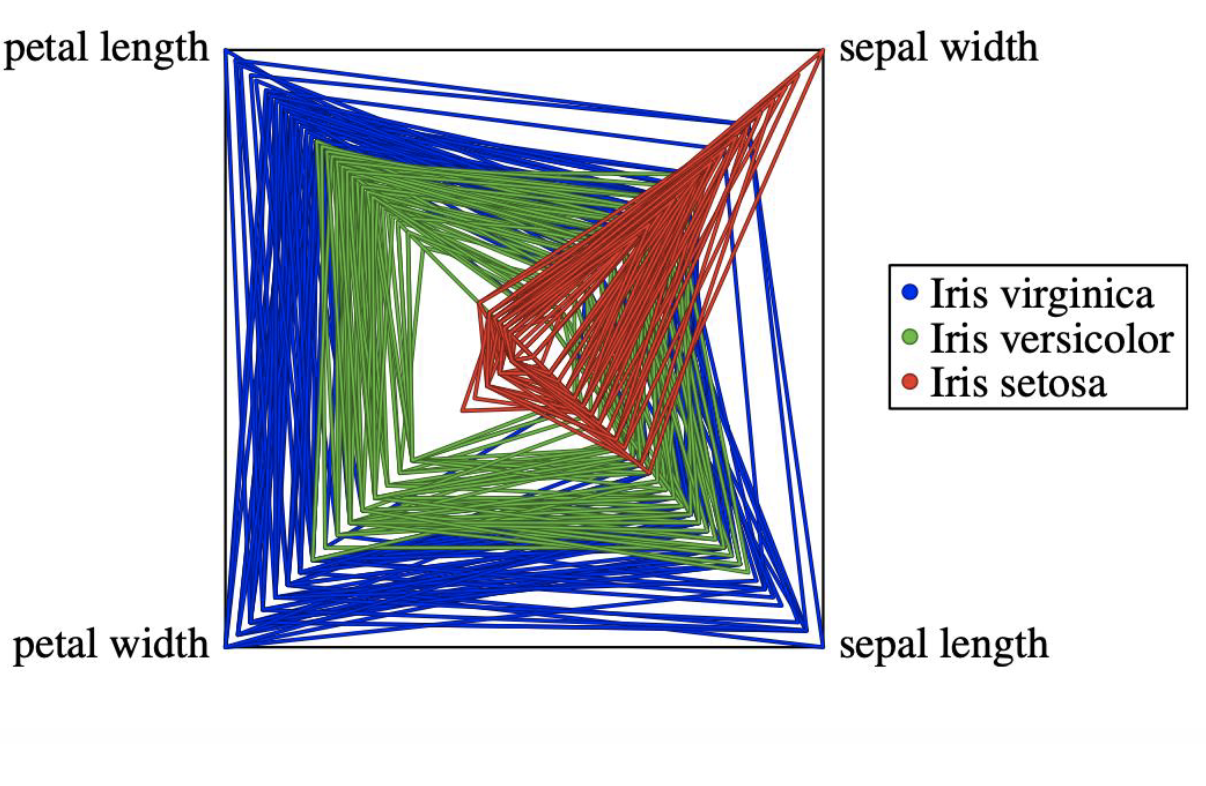
\includegraphics[width=\textwidth]{img/radar plot.png}
        \caption{A radar plot.}
    \end{minipage}
    \hfill
    \begin{minipage}[b]{0.43\textwidth}
        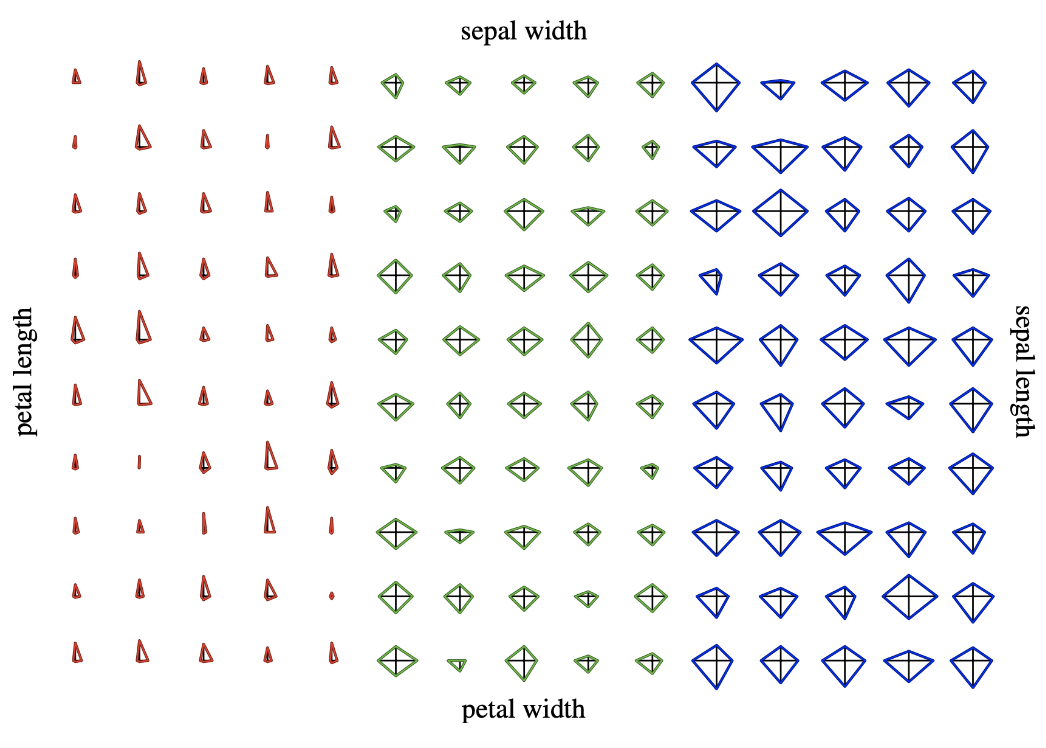
\includegraphics[width=\textwidth]{img/star plot.png}
        \caption{A star plot.}
    \end{minipage}
\end{figure}

\newpage

\section{Correlation analysis}

Correlation analysis is a popular technique for analyzing relationships between pairs of variables. For continuous variables, correlation is defined using \textbf{Pearson's correlation coefficient}.

\BoxDef{Pearson's correlation coefficient}{
Pearson's correlation coefficient between two variables is calculated as:
    \begin{equation*}
        \textit{corr}(x,y) = \dfrac{\textit{cov}(x,y)}{\sigma(x) \sigma(y)} = \dfrac{\sum_{i=1}^n (x_i - \textit{mean}(x))(y_i - \textit{mean}(y))}{(n-1) \sigma(x) \sigma(y)}
    \end{equation*}
}

The value of this coefficient lays between -1 and 1. When $\textit{corr}(x,y) = 1$, the two variables have a perfect positive correlation, else if $\textit{corr}(x,y) = -1$, the two variables have perfect negative correlation. Correlation can also be graphically visualized by using an appropriate plot, called \textbf{correlation matrix}.

\begin{figure}[h]
    \centering
    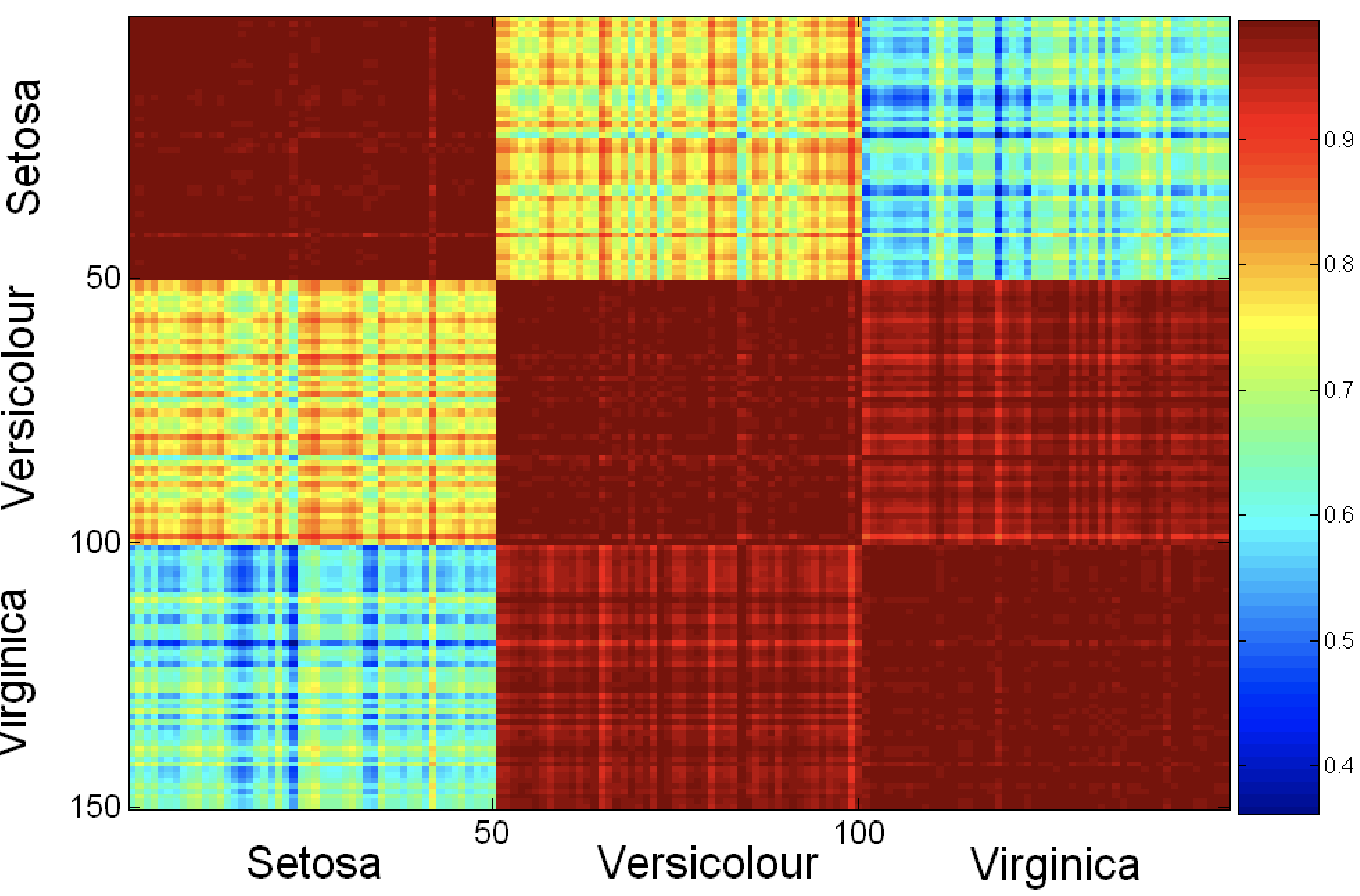
\includegraphics[width=0.4\linewidth]{img/correlation matrix.png}
    \caption{A correlation matrix.}
\end{figure}